\chapter{Design} \label{chap:design}

%\version{v1.10.2015}

\section*{}

In this chapter, MS/PhD system is observed each feature associated to its design.

\section{System Architecture}
This system is based on a two tier architecture. The first layer is the system with which the user interacts through a rich GUI. The second tier is the logical layer in which processing is carried out and quantifying of errors takes place.
Web Based MS/PHD Thesis System is divided into following components
\begin{itemize}
\item MS/PHD Thesis system is totally web base application.
\item The main functionality is system is students submit their proposal/Thesis through a web portal.
\item Database that contain the information about students.
\item Through web component user will be able to see the result of proposal/Thesis.
\end{itemize}

\section{Design Constraints}
The main emphasis of developing this application is make a paper free thesis system in university.Students submit their proposal/thesis through online portal.Develop this application using C\# interface thus make certain changes in interface methodology is main constraint. Providentially, using ASP.NET and oracle database, can achieve the desired objective.

\section{Design Methodology}
We will use procedural/structural approach to complete processing and design of the system, which will surely explain the core design of the automated thesis system.
The system will have following procedures
\begin{enumerate}
\item Student will register themselves for thesis.
\item After registering they will get email password of thesis web portal.
\item Where students can select their supervisor.
\item After selecting a supervisor students can easily send their proposal/thesis. 
\item And there is also a Administration panel where Admin access these student records.
\item After getting student records in Administration panel Admin will send the specific student record to corresponding supervisor.
\item Supervisor examine the specific record send back to Administration panel.
\item So Admin display the result of the student in student panel.
\item Interface will be simple and students and faculty members will enjoy the interaction with system.
\end{enumerate}  


\section{High Level Design}

The below given designs shows how this system will designed.
Figure \ref{fig:UsecaseDiagram} shows the working of system. 
	\begin{figure}[ht]
\centering
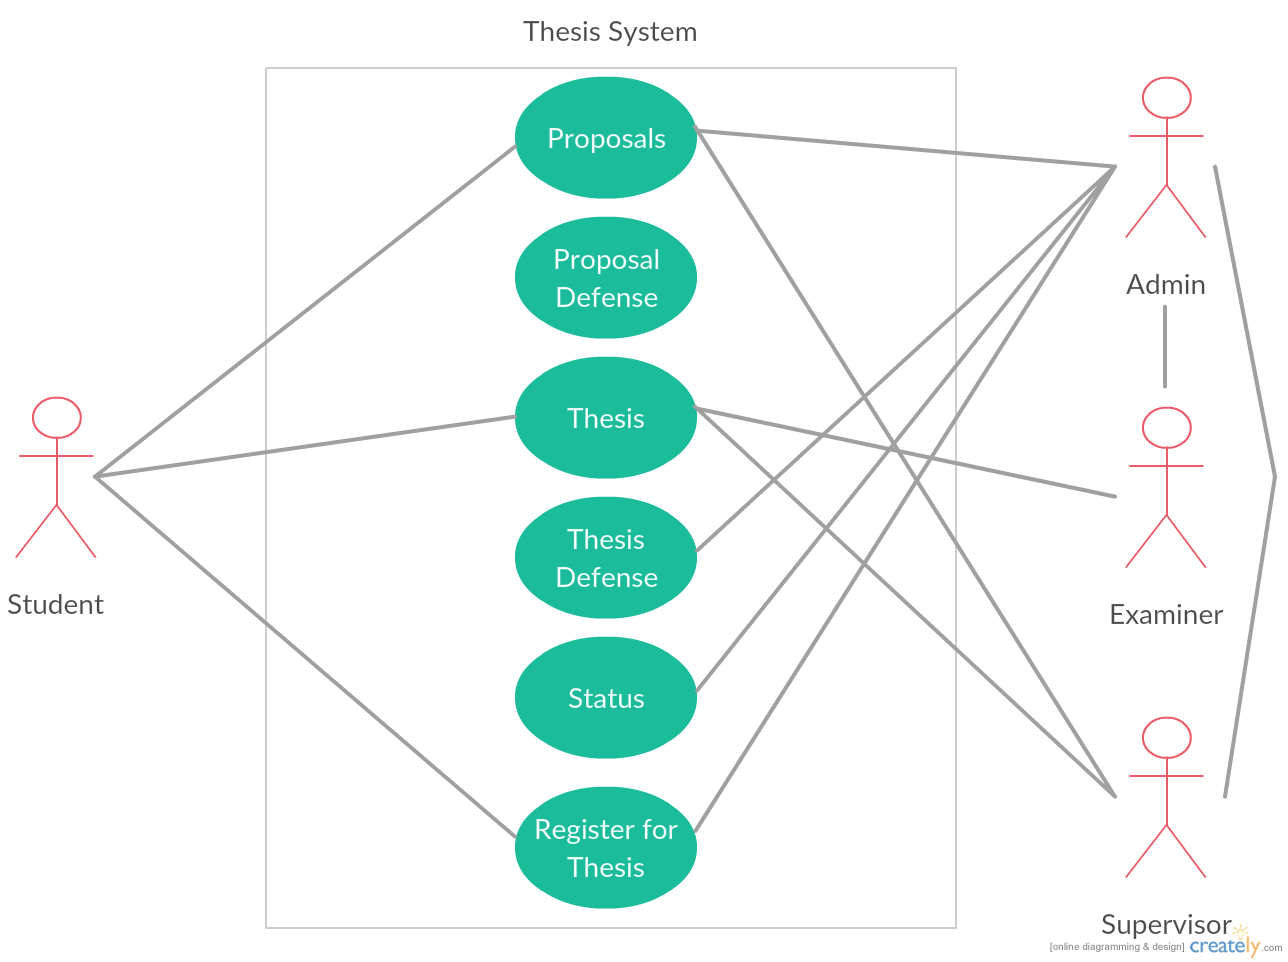
\includegraphics[scale=0.2]{UsecaseDiagram}
\caption{Use-Case Diagram}
\label{fig:UsecaseDiagram}
\end{figure}
\par This use-case diagram basically shows the user's interaction with this application that how user interact with this application. Shows different access levels and functionality of application that user interacts with which use-case.

\par This section describes in further detail elements discussed in the Architecture. Typical viewpoints are: 
\begin{enumerate}
	\item   Conceptual View: In Figure \ref{fig:ComponentDiagm} shows the logical functional elements of the system.  Each component represents a similar grouping of functionality.
	\begin{figure}[ht]
\centering
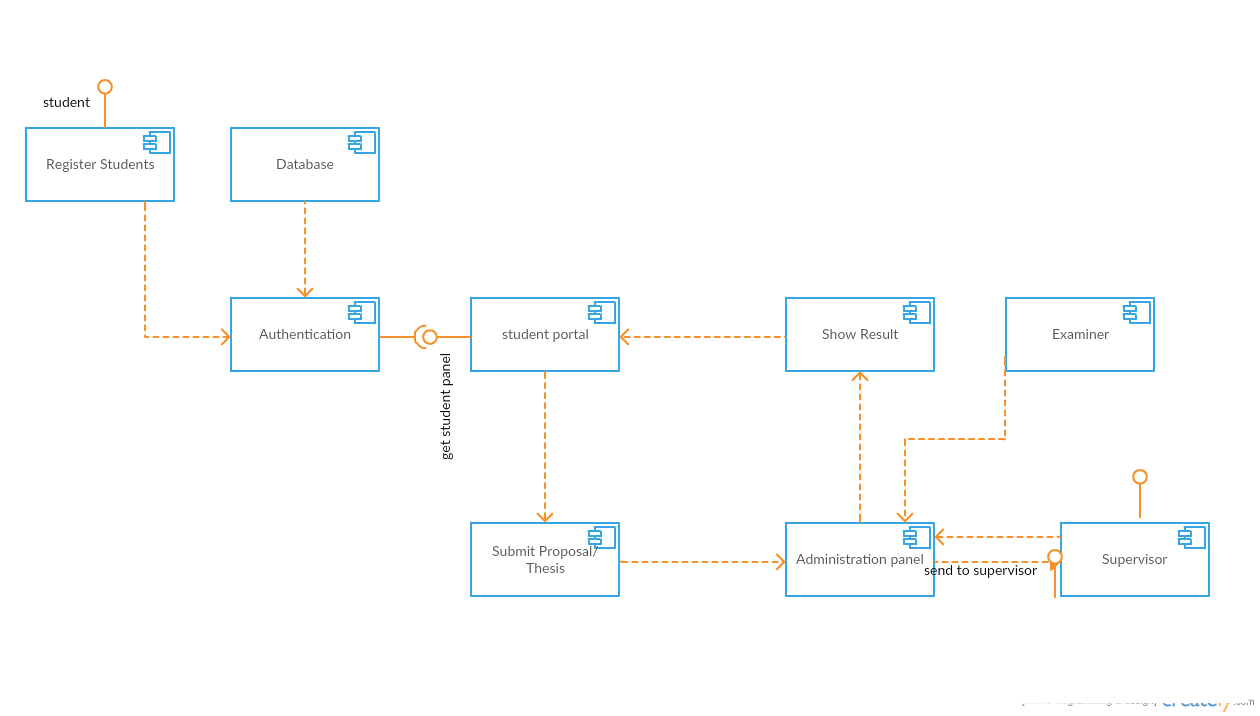
\includegraphics[scale=0.3]{ComponentDiagm}
\caption{Component Diagram}
\label{fig:ComponentDiagm}
\end{figure}

\end{enumerate}
\enlargethispage{-\baselineskip}
\section{Low Level Design}

\par Low level design of the application shows the different layers and shows at which layer which type of operation is perform. Data layer describes which type of data is used, Data access layer describes how data is accessed, Service layer illustrate the service provided to ADD, Business layer shows the complete operation performed by ADD and the last presentation layer illustrate the user interaction with ADD and different user interfaces.

\section{GUI Design}
The GUI of a system requires to be simple and user friendly. Since our designed system will be used by students and faculty members instead of computer scientist, therefore the GUI had to be very user friendly but extremely comprehensive. The best thing about our GUI design is that that it guides the user through step by step by going one activity to another activity. This chapter will explain the graphical user interface of the system. As the core objective of this system is to be used. So we need to design it simple, relevant and user friendly. By taking advantage of an individual suggestions impression, I am designing graphical user interface quite simple yet appealing. All of us use linear page layout for most styles as well as appropriate page layout.
\begin{figure}[ht]
\centering
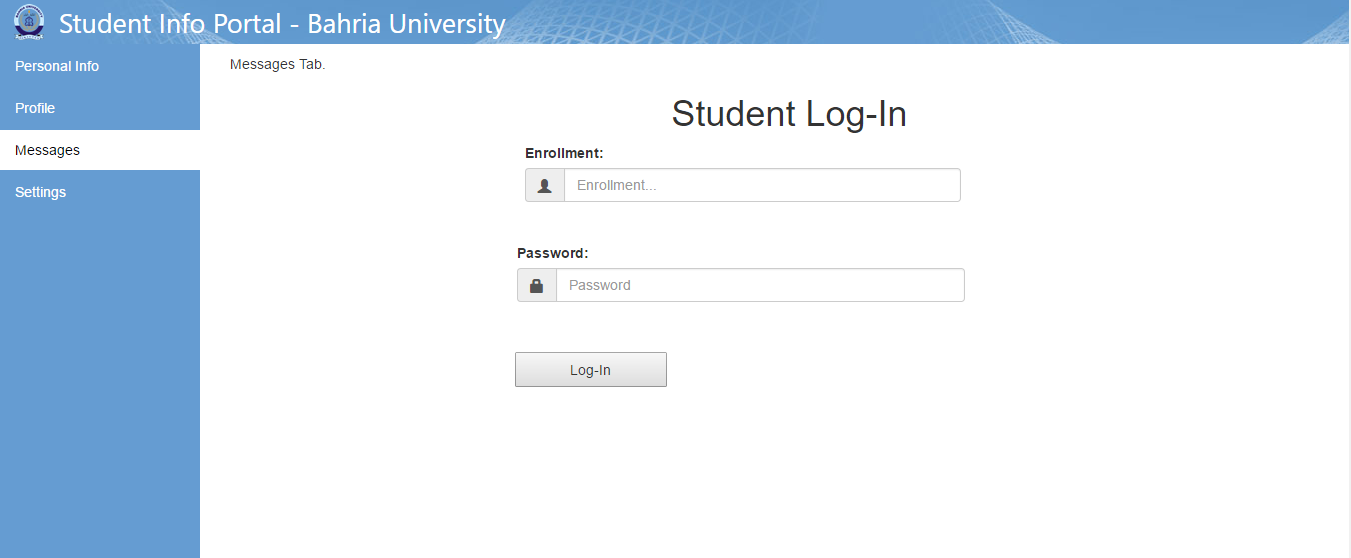
\includegraphics[scale=0.5]{first}
\caption{First User Interface}
\label{fig:first}
\end{figure}


